\documentclass[tikz, border=5pt]{standalone}
\usetikzlibrary{decorations.pathreplacing}

\begin{document}
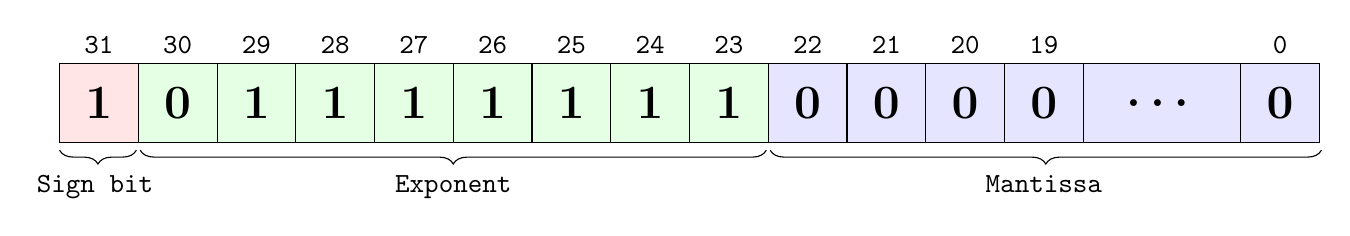
\begin{tikzpicture}

    % Colors
    \fill [red!10] (0, 0) rectangle (1, 1);
    \fill [green!10] (1, 0) rectangle (9, 1);
    \fill [blue!10] (9, 0) rectangle (16, 1);

    % Bozes
    \foreach \i in {0,...,12} {
            \draw (\i, 0) rectangle (\i + 1, 1);
        }
    \draw (15, 0) rectangle (16, 1);
    \draw (13, 0) rectangle (15, 0);
    \draw (13, 1) rectangle (15, 1);

    % Bits
    \node at (0.5, 0.5) {\LARGE \textbf 1};
    \node at (1.5, 0.5) {\LARGE \textbf 0};
    \node at (2.5, 0.5) {\LARGE \textbf 1};
    \node at (3.5, 0.5) {\LARGE \textbf 1};
    \node at (4.5, 0.5) {\LARGE \textbf 1};
    \node at (5.5, 0.5) {\LARGE \textbf 1};
    \node at (6.5, 0.5) {\LARGE \textbf 1};
    \node at (7.5, 0.5) {\LARGE \textbf 1};
    \node at (8.5, 0.5) {\LARGE \textbf 1};
    \node at (9.5, 0.5) {\LARGE \textbf 0};
    \node at (10.5, 0.5) {\LARGE \textbf 0};
    \node at (11.5, 0.5) {\LARGE \textbf 0};
    \node at (12.5, 0.5) {\LARGE \textbf 0};
    \node at (14, 0.5) {\LARGE \textbf \dots};
    \node at (15.5, 0.5) {\LARGE \textbf 0};

    % Positions
    \node [above] at (0.5, 1) {\texttt{31}};
    \node [above] at (1.5, 1) {\texttt{30}};
    \node [above] at (2.5, 1) {\texttt{29}};
    \node [above] at (3.5, 1) {\texttt{28}};
    \node [above] at (4.5, 1) {\texttt{27}};
    \node [above] at (5.5, 1) {\texttt{26}};
    \node [above] at (6.5, 1) {\texttt{25}};
    \node [above] at (7.5, 1) {\texttt{24}};
    \node [above] at (8.5, 1) {\texttt{23}};
    \node [above] at (9.5, 1) {\texttt{22}};
    \node [above] at (10.5, 1) {\texttt{21}};
    \node [above] at (11.5, 1) {\texttt{20}};
    \node [above] at (12.5, 1) {\texttt{19}};
    \node [above] at (15.5, 1) {\texttt{0}};

    %% IEEE 754 standard
    % Signed bit label
    \draw [decorate, decoration={brace, amplitude=5pt}] (1-0.025, -0.1) -- (0, -0.1);
    \node [below] at (0.45, -0.3) {\texttt{Sign bit}};

    % Exponent label
    \draw [decorate, decoration={brace, amplitude=5pt}] (9-0.025, -0.1) -- (1+0.025, -0.1);
    \node [below] at (5, -0.3) {\texttt{Exponent}};

    % Mantissa label
    \draw [decorate, decoration={brace, amplitude=5pt}] (16+0.025, -0.1) -- (9+0.025, -0.1);
    \node [below] at (12.5, -0.3) {\texttt{Mantissa}};

\end{tikzpicture}
\end{document}
